\documentclass{article}

% Symbols
%\usepackage{recycle}
\usepackage{amsfonts, amsthm}
\usepackage{upgreek}
\usepackage{physics}
\usepackage{cancel}
\usepackage{amssymb, latexsym, amsmath}

% Proof
\renewcommand*{\proofname}{\textbf{Demostraci\'on:}}

% Graphics
\usepackage{graphicx}
\usepackage{pgf}

% Color a letras.
%\usepackage[usenames,dvipsnames,svgnames,table]{xcolor}

% Tikz
\usepackage{tkz-graph}
\usepackage{tikz}
\usetikzlibrary{arrows,automata}
\usepackage{tikz}
\usetikzlibrary{arrows,automata}
% Def. Dr. César.
\usetikzlibrary{shapes,calc}
\tikzstyle{edge}=[shorten <=2pt, shorten >=2pt, >=stealth, line width=1.1pt]
\tikzstyle{blueE}=[shorten <=2pt, shorten >=2pt, >=stealth, line width=1.5pt, blue]
\tikzstyle{blackV}=[circle, fill=black, minimum size=6pt, inner sep=0pt, outer sep=0pt]
\tikzstyle{blueV}=[circle, fill=blue, draw, minimum size=6pt, line width=0.75pt, inner sep=0pt, outer sep=0pt]
\tikzstyle{redV}=[circle, fill=red, draw, minimum size=6pt, line width=0.75pt, inner sep=0pt, outer sep=0pt]
\tikzstyle{redSV}=[semicircle, fill=red, minimum size=3pt, inner sep=0pt, outer sep=0pt, rotate=225]
\tikzstyle{blueSV}=[semicircle, fill=blue, minimum size=3pt, inner sep=0pt, outer sep=0pt, rotate=225]
\tikzstyle{blackSV}=[semicircle, fill=black, minimum size=3pt, inner sep=0pt, outer sep=0pt, rotate=225]
\tikzstyle{vertex}=[circle, draw, minimum size=6pt, line width=0.75pt, inner sep=0pt, outer sep=0pt]

% Margins
\addtolength{\voffset}{-1cm}
\addtolength{\hoffset}{-1cm}
\addtolength{\textwidth}{2cm}
\addtolength{\textheight}{2cm}

%Header-Footer
\usepackage{fancyhdr}
\renewcommand{\headrulewidth}{1pt}

\newcommand{\set}[1]{%
  \left\{ #1 \right\}%
}

%\pagenumbering{gobble} -- Este comando
%                       -- quita el número de página.
\footskip = 50pt
\renewcommand{\headrulewidth}{1pt}

\pagestyle{fancyplain}

\begin{document}
\title{UNIVERSIDAD AUT\'ONOMA DE M\'EXICO\\ Facultad de Ciencias}
\author{Autores:
  \\ Fernanda Villaf\'an Flores
  \\ Fernando Alvarado Palacios
  \\ Adri\'an Aguilera Moreno}
\date{}
\maketitle
\begin{center}
  \includegraphics[scale=0.20]{../Imagen/Portada.jpg}\\[0.4cm]
  \Large
  \bf{Gr\'aficas y Juegos}
  \normalsize
\end{center}
\newpage
\fancyhead[r]{ Gr\'aficas y Juegos 2022-1}
%%%%%%%%%%%%%%%%%%%%%%%%%%%%%%%%%%%%%%%%%%%%%%%%%%%%%
\section*{\LARGE{Tarea 6}}
\begin{enumerate}
\item Sea $G$ una gr\'afica conexa no euleriana.   Demuestre que
  las siguientes afirmaciones son equivalentes.
  \begin{enumerate}
  \item Hay un paseo euleriano en $G$.

  \item Hay exactamente dos v\'ertices de grado impar en $G$.

  \item Existe una familia de ciclos ajenos por aristas dos
    a dos $\{ C_i \}_{i=1}^k$ y un paseo $P$ tal que
    $E_G = E_P \cup \bigcup_{i=1}^k E_{C_i}$.
  \end{enumerate}

  \begin{proof}
    Sea $G$ una gráfica.

    Probaremos las siguientes implicaciones:
    \begin{itemize}
    \item $(a) \Longrightarrow (b)$.

      Sea $P$ un paseo euleriano en $G$.

      Como $G$ es conexa, podemos hacer adyacentes al vértice inicial y al vértice final de $P$. Esto implica que tenemos un \textbf{paseo cerrado} y por tanto, tenemos un \textbf{circuito euleriano}.

      Así, obtenemos que $G$ es una gráfica euleriana.

      De aquí, notemos que todos los vértices de la gráfica euleriana tienen grado par (\textit{por propiedades de gráficas eulerianas}) y, si borramos la arista que une al vértice inicial y al vértice final de $P$, obtenemos que el grado de dichos vértices disminuye en $1$.

      Esto implica que ambos vértices ahora tienen grado impar (ya que \textit{número par $-$ número impar $=$ número impar}).

      Por lo tanto, dichos vértices son los únicos dos vértices de grado impar en $G$.

    \item $(b) \Longrightarrow (c)$.

      Como ya probamos que $G$ es una gráfica euleriana, \textit{por propiedades} sabemos que $G$ tiene una \textbf{descomposición en ciclos}, digamos $C_{1}, C_{2}, \cdots, C_{k}$. Y además por el inciso $(a)$, sabemos que existe un paseo $P$ en $G$ el cuál (\textit{por hipótesis}) tiene exactamente dos vértices de grado impar.

      Entonces tenemos que:
      \begin{equation*}
        \begin{split}
          E_{G}
          & = \bigcup_{i=1}^{k} E_{C_{i}} \cup E_{P} \\
          & = E_{P} \cup \bigcup_{i=1}^{k} E_{C_{i}}
        \end{split}
      \end{equation*}

    \item $(c) \Longrightarrow (a)$.

      Esto es inmediato ya que \textit{por hipótesis}, existe un paseo $P$ tal que:
      $$E_{G} = E_{P} \cup \bigcup_{i=1}^{k} E_{C_{i}}$$

      En particular si $G$ no tiene ciclos, es decir, $\displaystyle \bigcup_{i=1}^{k} E_{C_{i}} = \emptyset$ tenemos que:
      \begin{equation*}
        \begin{split}
          E_{G}
          & = E_{P} \cup \bigcup_{i=1}^{k} E_{C_{i}} \\
          & = E_{P} \cup \emptyset \\
          & = E_{P}
        \end{split}
      \end{equation*}

      Así, si $E_{G} = E_{P}$ implica que hay un paseo euleriano en $G$ (por definición de \textbf{paseo euleriano}).

      Por lo tanto, queda demostrado que las afirmaciones son equivalentes.
    \end{itemize}
  \end{proof}

\item Sea $D$ una digr\'afica conexa. Demuestre que $D$ es
  euleriana si y s\'olo si  para cada $v \in V_D$, se tiene
  $d^+(v) = d^-(v)$.

  \begin{proof}
    \begin{itemize}
    \item $\Longrightarrow$.

      Sea $D$ una digráfica conexa e eucliriana $\rightarrow$ Por definición de gráfica eucliriana existe un circuito euclidiano que une a todos los vértices, llamémosle $C$ a este circuito.

      Entonces, sea $x$ perteneciente a $V_D$ el inicio de este circuito.

      $\rightarrow$ $C = (x,v_i, v_{i+1}, \cdots, v_{i+n}, u)$ con $i$ y $n$ pertenecientes a los naturales.

      Como todos los vértices son consecutivos, notemos que cada vértice de $C$ es cola y cabeza para dos flechas distintas en el circuito $\rightarrow$ para todo $V_k$ que pertenece a $C$ existe $d^+$ y $d^-$ que une a $V_k$ con sus vértices adyacentes $V_{k-1}$ y $V_{k+1}$.

      Así, cada vértice de la trayectoria $C$ tendrá  una ``arista" $d^+$ y una $d^-$ (ya que $D$ es par y por construcción de $C$).

      Por lo tanto, $d^+ = d^-$ ya que para todo vértice de $D$ se pueden sumar el número de veces que aparecen en la trayectoria $C$ y preservará la igualdad anterior.

    \item $\Longleftarrow$.

      Sea $D$ conexa y para toda $v$ que pertenece a $V_D$ se tiene que $d^+ = d^- \rightarrow$ para toda $v$ que pertenece a $V_D$, existe al menos una $d^+$ y una $d^-$.

      Por lo que para todo $v$ que pertenece a $V_D$, $v$ es mayor igual a $2$. Pero el grado de $v$ siempre debe ser par, ya que tenemos la igualdad $d^+ = d^- \rightarrow$ $D$ es par.

      Por lo tanto, por teorema visto en clase tenemos que $D$ es una gráfica eucliriana.
    \end{itemize}
  \end{proof}
%%%%%%%%%%%%%%%%%%%%%%%%%%%%%%%%%%%%%%%%%%%%%% Ejercicio 3
\item La digr\'afica de {\em de Bruijn-Good} $BG_n$ tiene como
  conjunto de v\'ertices al conjunto de todas las sucesiones
  binarias de longitud $n$, y donde el v\'ertice $a_1 a_2
  \cdots a_n$ es adyacente al v\'ertice $b_1 b_2 \cdots b_n$
  si y s\'olo si $a_{i+1} = b_i$ para $1 \le i \le n-1$.  Demuestre
  que $BG_n$ es una digr\'afica euleriana de orden $2^n$ y
  di\'ametro dirigido $n$.

  \begin{proof}
    Sabemos que dado $2$ vértices $v = a_1a_2 \dotsm a_n$ y
    $u = b_1b_2 \dotsm b_n$, estos son adyacentes si $1 \leq i \leq n -1$,
    luego $BG_n$ es $4$-regular, pues existen $4$ maneras de elegir
    vértices adyacentes a algún $x \in V_{BG_n}$. Veamos un ejemplo
    general de lo antes mencionado: Sean $x = a \dotsm b$ e $y = c \dotsm d$
    donde $x, y \in V_{BG_n}$ y $a,b,c,d \in \{0,1\}$, así $xy \in E_{BG_n}$
    si $\dotsm b = c \dotsm$, como podemos tomar $c,d$ como $OR_2^2 = 2^2 = 4$,
    entonces cada vértice tiene grado $4$, exactamente dos aristas de
    ``\textit{llegada}'' y dos de ``\textit{salida}'' inciden en $x$.
    Como $G$ es $4$-regular, entonces es par y por el teorema de caracterización
    de las gráficas eulerianas concluimos que $G$ es euleriana.

    Por combinatoria sabemos que $OR_2^n = 2^n$ [ordenaciones con repetición]
    y este es justo el orden de $BG_n$.

    Sabemos por la definición de distancia entre dos vértices que esta es la
    mínima trayectoria entre los vértices. Sea $x = 0 \dotsm 0$ e $y = 1 \dotsm 1$
    (con tantos 0's y 1's como $n$ en $BG_n$) y a su vez $xy$-trayectoria
    (caso análogo $yx$-trayectoria) es de longitud $n$, pues el rabo [cola] o vértice
    donde se esta ubicado, que en un inicio es $x$, incide en el vértice que sustituya al
    ``$1$'' más a la derecha en la cadena (nodo) que se ubique por un ``$0$'', así
    habrá exactamente $n$ aristas en $xy$ o $n +1$ vértice en $xy$, luego $xy$ es
    de la distancia de longitud máxima (esto no quiere decir que sea la única)
    entre todas las distancias, pues se hacen al menos $n$ cambios en la cadena (que
    tiene $n$ dígitos tomados entre $1$'s y $0$'s) $x$ para ``\textit{llegar}'' a $y$.
    Luego, por definición de diámetro en una digráfica, el diámetro de $BG_n$ es $n$.

    De lo anterior se concluye la demostraci\'on.
  \end{proof}
   \newpage
  %%%%%%%%%%%%%%%%%%%%%%%%%%%%%%%%%%%%%%%%%%%%%% Ejercicio 4
\item Demuestre que existe una forma de ordenar todas las fichas
  de domin\'o en un ciclo (respetando las reglas del juego).
  ?`C\'omo generalizar\'ia este resultado para domin\'os con
  $n$ puntos? (el domin\'o est\'andar es el de $6$ puntos).

  \begin{proof}
    A continuación se muestra una manera de ordenar las fichas de dominó de
    tamaño estándar en un ciclo:

    \begin{center}
      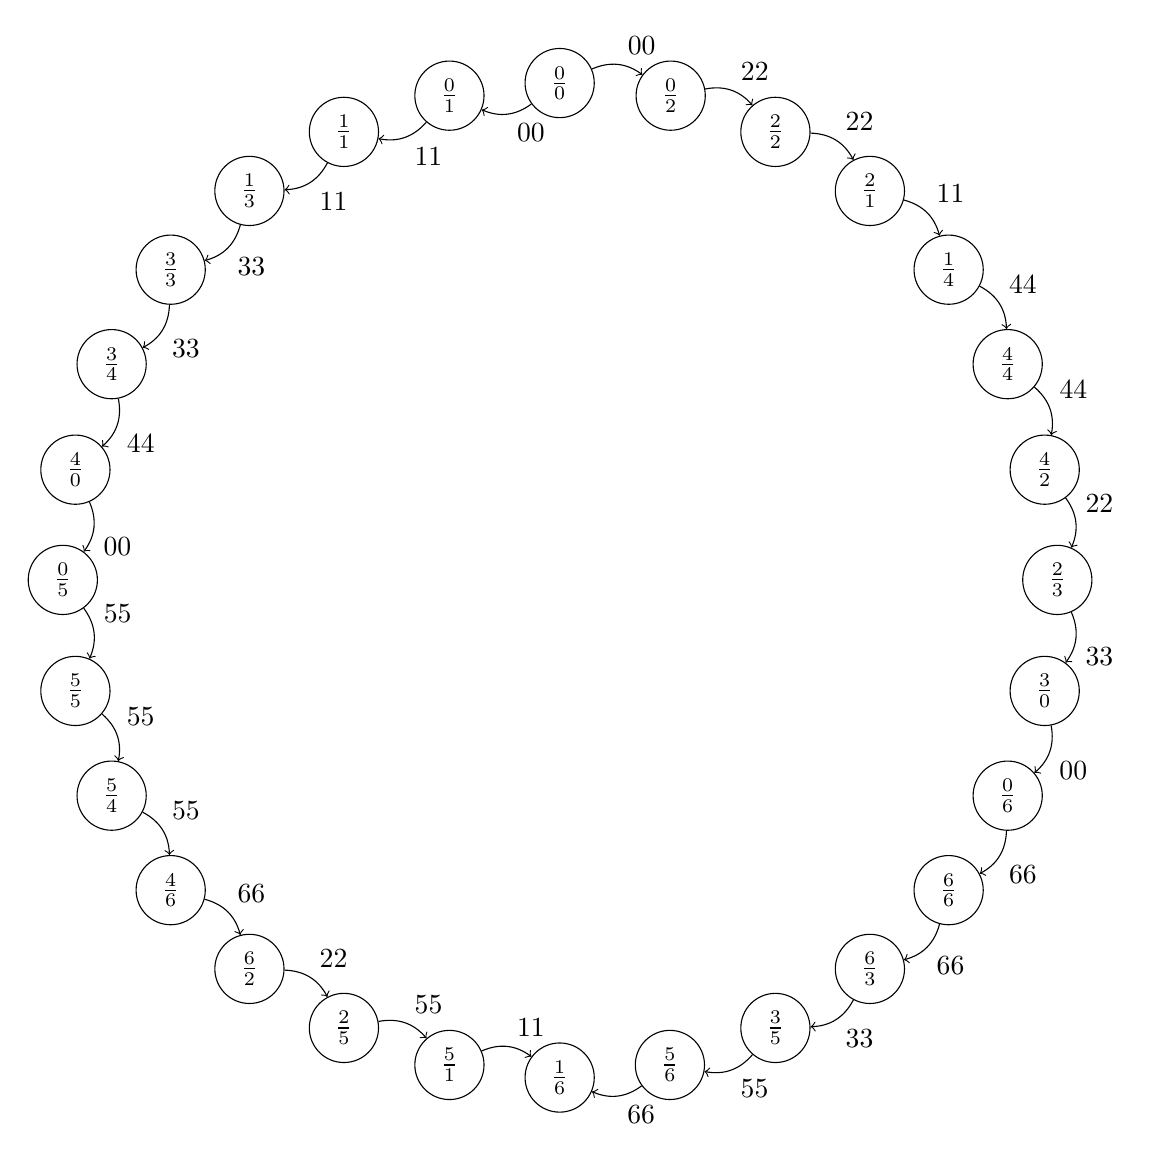
\begin{tikzpicture}[->, node distance = 3cm, auto]

        \node[state](v1)   at(0,  0)         {$\frac{6}{3}$};
        \node[state](v2)   at(1,  1)         {$\frac{6}{6}$};
        \node[state](v3)   at(1.75,  2.2)    {$\frac{0}{6}$};
        \node[state](v4)   at(2.22,  3.53)   {$\frac{3}{0}$};
        \node[state](v5)   at(2.38,  4.94)   {$\frac{2}{3}$};
        \node[state](v6)   at(2.22,  6.34)   {$\frac{4}{2}$};
        \node[state](v7)   at(1.75,  7.68)   {$\frac{4}{4}$};
        \node[state](v8)   at(1,     8.88)   {$\frac{1}{4}$};
        \node[state](v9)   at(0,     9.88)   {$\frac{2}{1}$};
        \node[state](v10)  at(-1.2,  10.63)  {$\frac{2}{2}$};
        \node[state](v11)  at(-2.53,  11.09) {$\frac{0}{2}$};
        \node[state](v12)  at(-3.94,  11.25) {$\frac{0}{0}$};
        \node[state](v13)  at(-5.34,  11.09) {$\frac{0}{1}$};
        \node[state](v14)  at(-6.68,  10.63) {$\frac{1}{1}$};
        \node[state](v15)  at(-7.88,  9.88)  {$\frac{1}{3}$};
        \node[state](v16)  at(-8.88,  8.88)  {$\frac{3}{3}$};
        \node[state](v17)  at(-9.63,  7.68)  {$\frac{3}{4}$};
        \node[state](v18)  at(-10.09, 6.34)  {$\frac{4}{0}$};
        \node[state](v19)  at(-10.25, 4.94)  {$\frac{0}{5}$};
        \node[state](v20)  at(-10.09, 3.53)  {$\frac{5}{5}$};
        \node[state](v21)  at(-9.63,  2.2)   {$\frac{5}{4}$};
        \node[state](v22)  at(-8.88,  1)     {$\frac{4}{6}$};
        \node[state](v23)  at(-7.88,  0)     {$\frac{6}{2}$};
        \node[state](v24)  at(-6.68, -0.75)  {$\frac{2}{5}$};
        \node[state](v25)  at(-5.34, -1.22)  {$\frac{5}{1}$};
        \node[state](v26)  at(-3.94, -1.38)  {$\frac{1}{6}$};
        \node[state](v27)  at(-2.54, -1.22)  {$\frac{5}{6}$};
        \node[state](v28)  at(-1.2,  -0.75)  {$\frac{3}{5}$};

        %%----------------------------------
        \path (v12)edge[bend left]node{$00$}(v11)
        (v12)edge[bend left]node{$00$}(v13)
        (v13)edge[bend left]node{$11$}(v14)
        (v11)edge[bend left]node{$22$}(v10)
        (v14)edge[bend left]node{$11$}(v15)
        (v10)edge[bend left]node{$22$}(v9)
        (v15)edge[bend left]node{$33$}(v16)
        (v9)edge[bend left]node{$11$}(v8)
        (v16)edge[bend left]node{$33$}(v17)
        (v8)edge[bend left]node{$44$}(v7)
        (v17)edge[bend left]node{$44$}(v18)
        (v7)edge[bend left]node{$44$}(v6)
        (v18)edge[bend left]node{$00$}(v19)
        (v6)edge[bend left]node{$22$}(v5)
        (v19)edge[bend left]node{$55$}(v20)
        (v5)edge[bend left]node{$33$}(v4)
        (v20)edge[bend left]node{$55$}(v21)
        (v4)edge[bend left]node{$00$}(v3)
        (v21)edge[bend left]node{$55$}(v22)
        (v3)edge[bend left]node{$66$}(v2)
        (v22)edge[bend left]node{$66$}(v23)
        (v2)edge[bend left]node{$66$}(v1)
        (v23)edge[bend left]node{$22$}(v24)
        (v1)edge[bend left]node{$33$}(v28)
        (v24)edge[bend left]node{$55$}(v25)
        (v28)edge[bend left]node{$55$}(v27)
        (v27)edge[bend left]node{$66$}(v26)
        (v25)edge[bend left]node{$11$}(v26);
        %%----------------------------------
      \end{tikzpicture}
    \end{center}
    donde $\frac{0}{0}$ es la ficha que no tiene puntos, $\frac{1}{5}$
    la ficha con uno y cinco puntos, y así de manera consecutiva. Las
    aristas indican como se van uniendo las fichas.

    Por el ejemplo anterior queda mostrado que existe una manera de ordenar
    las fichas en un dominó de $6$ puntos en forma de ciclo. Para mostrar
    este resultado de manera general, hay que notar que necesitamos una
    condición necesaria, esta es, el dominó debe de ser de $n = 2 \cdot k$
    [$k \in \mathbb{N}$] puntos, pues en caso contrario no podemos obtener
    un ciclo, ya que existirán $2k +1$ fichas con el valor de $0$ en alguna
    posición, \textit{i.e.}, una ficha que tenga cero puntos en alguna de
    sus ``\textit{caras}''\footnote{No sé como se les llama a las dos partes
      que tiene una ficha de dominó, nunca había jugado dominó jejeje.}, y por
    paridad no podremos agrupar en parejas a las fichas que tengan cero puntos
    en alguna de sus ``\textit{caras}''. Luego el dominó cumple con
    $n = 2 \cdot k$, y cada vértice [\textit{ficha de dominó}] tiene, a lo
    más, grado $2$. Nótese que la cantidad total de fichas es $\frac{n \cdot (n +1)}{2}$
    y cada ficha tiene dos ``\textit{caras}'', luego hay
    $n \cdot (n +1) = 2 \cdot (k^2 + k)$ ``\textit{caras}'', lo que es una cantidad
    par. Luego, veamos que pasa cuando:
    \begin{itemize}
    \item[$\cdot$)] $n$ es par, entonces las $n$ fichas que contengan $n$ puntos en
      alguna de sus ``\textit{caras}'' son una cantidad par [el total de estas], la idea
      anterior se puede aplicar para cualquier $n_i$ con $i \in \{1, \dotsm, n\}$ si $n_i$
      es una cantidad par. Además, hay una cantidad par de fichas con caras igual a $n_i$
      puntos, pues las fichas con puntos mayor a $n_i$ contienen alguna con una cara igual
      a $n_i$ puntos, luego estas son $n - n_i$ y si les sumamos las $n_i$ antes contadas
      tenemos que hay $n$ fichas que cumplen lo antes mencionado.

    \item[$\cdot$)] Las fichas impares (las que tengan puntos impares, un ejemplo serían
      todas las fichas que tienen $3$ puntos en una de sus caras) son una cantidad par, pues
      si hay una ficha con $m = 2p +1$ [$p \in \mathbb{N}$] puntos, como $n$ es par y es la
      mayor cantidad de puntos que podrá tener una de las ``\textit{caras}'' en cualquier ficha,
      entonces hay al menos $n -m$ fichas que contienen $m$ puntos en una de sus ``\textit{caras}''
      y la otra ``\textit{cara} contiene al menos $m +1$ puntos, \textit{i.e.},
      \begin{eqnarray*}
        n - m &=& 2 \cdot k - (2 \cdot p +1)\\
        &=& 2 \cdot (k - p) + 1
      \end{eqnarray*}
      con $k > p$. Lo anteior es impar [$n -m$] y por paridad \textit{impar} $+$ \textit{impar}
      es par y concluimos que las fichas con $m$ puntos en al menos una de sus caras son una cantidad
      par, otra manera de verlo es que $(n -m) + m = n$ y hay justo $n$ fichas con al menos una de
      sus caras igual a $m$ puntos.
    \end{itemize}

    Como en cualquiera de los casos anteriores hay una cantidad par de fichas, entonces podemos agrupar
    conjuntos [aristas] de orden $2$ con las fichas [vértices] y obtendremos una gráfica par, pues cada
    ficha se relacionará con exactamente $2$, luego, los ordenes $n$ en el dominó, siempre que $n$ sea
    par, forman gráficas eulerianas, luego por el teorema de caracterización de gráficas eulerianas tenemos
    que esta es un ciclo.
  \end{proof}
\item Sean $G$ una gr\'afica euleriana no trivial
  y $u \in V_G$. Demuestre que todo paseo en $G$
  que inicia en $u$ se puede extender a un circuito
  euleriano si y s\'olo si $G-u$ es ac\'iclica.

  \begin{proof}
    Sean $G$ una gr\'afica euleriana no trivial y $u \in V_{G}$.

    Procedemos por doble implicación.

    \begin{itemize}
      \item $\Longrightarrow$.

        Suponemos que todo paseo en $G$ que inicia en $u$ se puede extender a un circuito euleriano.

        Demostraremos que $G-u$ es ac\'iclica.

        \textbf{Procedemos por contradicción.}

        Sea $P$ un circuito euleriano de $G$.

        Supongamos que $G-u$ no es ac\'iclica. Esto implica que existe un ciclo $C$ en $G-u$.

        Ahora, como $G$ es una gráfica euleriana, en particular es par, entonces $G - E_{C}$ debe ser par. Notemos que el vértice $u$ no pertenece a los vértices del ciclo $C$, lo que implica que $u$ no es adyacente a ningún vértice del ciclo $C$.

        De lo anterior tenemos que $u \in V_{P}$ y entonces, $P$ empieza y termina en $u$. Así, como todos los vértices adyacentes a $u$ están en $P$ implica que $P$ no se puede extender a un circuito euleriano !!!

        La contradicción yace de suponer que $G - u$ no es acíclica, por tanto, $G - u$ es acíclica.

      \item $\Longleftarrow$.

        Suponemos que $G-u$ es ac\'iclica.

        Demostraremos que todo paseo en $G$ que inicia en $u$ se puede extender a un circuito euleriano.

        Como $G - u$ es acíclica, implica que todo ciclo $C$ en $G$ contiene al vértice $u$. De aquí, entonces tenemos que todo ciclo $C$ en $G$ empieza y termina en $u$ (pues sabemos que un ciclo empieza y termina en el mismo vértice, es decir, es cerrado).

        Ahora, como cada ciclo en $G$ no comparte ninguna arista (porque $G$ es una gráfica euleriana), \textit{por propiedades} sabemos que existe una familia de ciclos $\bigg\{ C_{i}\bigg\}_{i = 1}^{k}$ y un paseo $P$ tal que:
        $$E_{G} = E_{P} \cup \bigcup_{i = 1}^{k} E_{C_{i}}$$

        Sea $u \in V_{P}$. Entonces se sigue que $P$ debe ser un paseo que inicia y termina en el mismo vértice (en este caso, $u$), lo que implica que $P$ es un paseo cerrado y por definición, $P$ sería un circuito euleriano.

        Por lo tanto, tenemos un paseo cualquiera en $G$ que empieza en $u$ y se puede extender a un circuito euleriano.
    \end{itemize}

    Por lo anterior, podemos concluir que todo paseo en $G$ que inicia en $u$ se puede extender a un circuito euleriano si y s\'olo si $G-u$ es ac\'iclica.
  \end{proof}
\end{enumerate}

\section*{Puntos Extra}
\begin{enumerate}
\item Una digr\'afica $D$ es {\em balanceada} si $|d^+(v) - d^-(v)|
  \le 1$, para cada $v \in V$.   Demuestre que toda gr\'afica tiene
  una orientaci\'on balanceada.

  \begin{proof}


    Sea G una grafica $\rightarrow$ G tendrá vertices de grado par o impar, sea x un vertice que no pertenezca a G, construiremos a $G^1$ parecida a G, con la diferencia de que todos los vértices G que sean impares estaran relacionados con el vértice X, por lo tanto, todos los vertices de nuestra nueva gráfica $G^1$ tendran grado par, por lo que $G^1$ sera una grafica G euleriana, lo que implica que tendra un circuito euleriano que empezara en el vector x y terminara en el vector x, $\rightarrow$ le podemos dar un orden a las aristas de $G^1$ mediante este ciclo (si $v_k$ es un vertice de $G^1$ para algun k natural  $\rightarrow$ de $v_{k-1}$ a $v_k$ tendremos una flecha  $d^-$ y de $v_{k}$ a $v_{k+1}$ tendremos una flecha $d^+$), ya que construimos la digrafica $G^1\rightarrow$ vamos a quitar las aristas ``ahora flechas" que agregamos hace un momento y ahora esta esta nueva digráfica será G $\rightarrow$ podemos notar que si los grados de los vértices de G eran pares $\rightarrow|d^+(v) - d^-(v)| = 0$ ``por construccion de $G^1$" y si los grados de los vertices eran impares $\rightarrow |d^+(v) - d^-(v)|=1$ (por construcción de la digráfica $G^1$).

    Por lo tanto, para todo vertice de la digrafica G tenemos que $|d^+(v) - d^-(v)| es menor igual que 1$ por lo tanto toda gráfica G tiene un orientación balanceada.

    \end{proof}

\item Una sucesi\'on circular $s_1 s_2 \cdots s_{2^n}$ de ceros
  y unos es llamada una {\em sucesi\'on de de Bruijn-Good}
  de orden $n$ si las $2^n$ subsucesiones $s_i s_{i+1} \cdots
  s_{i+n-1}$, $1 \le i \le 2^n$ (con los sub\'indices tomados
  m\'odulo $2^n$ son distintas, y por lo tanto constituyen todas
  las posibles sucesiones binarias de longitud $n$.   Por ejemplo,
  la sucesi\'on $00011101$ es una una sucesi\'on de de Bruijn-Good
  de orden tres.   Muestre como encontrar un de estas sucesiones
  para cualquier orden $n$ utilizando un circuito euleriano dirigido
  en la gr\'afica de de Bruijn-Good $BG_{n-1}$. Justifique su
  respuesta.

\item Sea $G$ una gr\'afica conexa, y sea $X$ el conjunto
  de v\'ertices de $G$ de grado impar.   Suponga que
  $|X| = 2k$, con $k \ge 1$.
  \begin{enumerate}
  \item Demuestre que hay $k$ paseos ajenos por
    aristas $Q_1, \dots, Q_k$ en $G$ tales que
    $E_G = \bigcup_{i=1}^k E_{Q_i}$.

  \item Deduza que $G$ contiene $k$ paseos ajenos
    por aristas que conectan a los v\'ertices de $X$
    en pares.
  \end{enumerate}
\end{enumerate}
\end{document}
